%
% Шаблон для ВКР бакалавра 2026
%

\documentclass[a4paper,12pt]{article}
\usepackage{vkriate}

% Настройки для окружений с подчеркиваниями для подписей и пр.
\setFRMfontencoding{T2A}
\setFRMdfontencoding{T2A}
% thanks to A.Starikov
\setFRMfontfamily{cmr}
\setFRMdfontfamily{ptm}
\setFRMdfontsize{10pt}

% задает длину поля для подписи на титульной странице
\newFRMfield{xtitlesign}{32mm}

% поле для факультета или кафедры
\newFRMfield{fcath}{65mm}

%имя файла с библиографией в формате BibTex
\addbibresource{rbiblio.bib}

\begin{document}

% счетчики страниц, рисунков, таблиц
\regtotcounter{page}
\regtotcounter{figure}
\regtotcounter{table}

\renewcommand{\refname}{\centerline{СПИСОК ИСПОЛЬЗОВАННЫХ ИСТОЧНИКОВ}} 
\renewcommand{\contentsname}{\centerline{СОДЕРЖАНИЕ}} 
%\renewcommand{\refname}{Список источников}  % По умолчанию "Список литературы" (article)
%\renewcommand{\bibname}{Литература}  % По умолчанию "Литература" (book и report)

% титульная страница
\thispagestyle{empty}
\begin{center} \small
\textbf{МИНИСТЕРСТВО НАУКИ И ВЫСШЕГО ОБРАЗОВАНИЯ\\ РОССИЙСКОЙ ФЕДЕРАЦИИ}\\
ФЕДЕРАЛЬНОЕ ГОСУДАРСТВЕННОЕ АВТОНОМНОЕ ОБРАЗОВАТЕЛЬНОЕ УЧРЕЖДЕНИЕ
ВЫСШЕГО  ОБРАЗОВАНИЯ\\
«Национальный исследовательский ядерный университет «МИФИ»\\
\textbf{Обнинский институт атомной энергетики} – \\
филиал федерального государственного автономного образовательного учреждения высшего\\
образования «Национальный исследовательский ядерный университет «МИФИ»\\
(ИАТЭ НИЯУ МИФИ)
\end{center}
%\vfill
\medskip

% Направление подготовки следует уточнять,
% магистры и бакалавры могут иметь разные наименования
\begin{center}
\begin{tabular}{rl}
Отделение & \useFRMfield{fcath}[\large Интеллектуальные кибернетические системы] \\ 
%Направление подготовки & \useFRMfield{fcath}[\large Информационные системы и технологии] \\ 
\end{tabular} 
\end{center}

\vfill

\large 

\begin{center}
\textbf{\Large Выпускная квалификационная работа --- } \\
\textbf{\Large бакалаврская работа}\\
	
	\medskip

{ \normalsize
по направлению подготовки  \textbf{09.03.02 Информационные  системы и технологии}\\

Направленность (профиль) \textbf{Информационные технологии}
}	
\vfill
\vfill
\medskip

\textbf{\Large 
		<<Полное наименование ВКР в соответствии с заданием>>
	}
	
\end{center}

\vspace{1cm}

\begin{center}
\begin{tabular*}{\textwidth}{p{78mm}p{33mm}p{64mm}}
	Выполнил:\\студент гр. ИС-Б22 & \useFRMfield{xtitlesign} & Студе~Н.Т.\\
	& & \\
% должность, научная степень руководителя
	Руководитель ВКР,\\доцент отделения ИКС, к.т.н. & \useFRMfield{xtitlesign} & Руководит~Е.Л. \\
	& & \\
	
	Нормоконтроль\\ доцент отделения ИКС, к.ф.-м.н. & \useFRMfield{xtitlesign} &  Качанов~Б.В. \\
	& & \\
	% Если нужно добавить консультанта - раскомментируйте две строчки ниже
	%Консультант ВКР бакалавра\\организация, должность, звание  & \useFRMfield{xtitlesign} & К.О.Нсультант\\
	%& & \\
%	Рецензент\\к.ф.-м.н.,   & \useFRMfield{xtitlesign} & В.А. Чепурко\\
	
	& & \\
	Выпускная квалификационная \\ работа допущена к защите & \useFRMfield{xtitlesign} &  \\
	& & \\
	Руководитель\\ образовательной программы \\
	09.03.02 Информационные системы и технологии\\
	канд. тех. наук  & \useFRMfield{xtitlesign} &Мирзеабасов~О.А. \\
	
\end{tabular*}
\end{center}

\vfill
\large

\begin{center}
Обнинск, 2026 г
\end{center}

\onehalfspacing

\pagebreak

% ГОСТ 7.32-2017 - нумерация страниц не проставляется только на титульной странице
% реферат
%\thispagestyle{empty}

\setcounter{page}{2}

\section*{\centering РЕФЕРАТ}

%\thispagestyle{empty} % страница реферата не нумеруется

Работа \total{page} стр., \total{table} табл., \total{figure} рис., \totalmycitecounts ист. 

КЛЮЧЕВЫЕ СЛОВА В ВЕРХНЕМ РЕГИСТРЕ

Текст реферата должен отражать:
\begin{itemize}
\item объект исследования;
\item предмет исследования;
\item цель работы;
\item метод или методологию проведения работы;
\item научную новизну исследования (для магистерских диссертаций);
\item практическую значимость результатов работы;
\item степень внедрения (при наличии справки о внедрении);
\item экономическую эффективность работы.
\end{itemize}
Текст реферата должен размещаться на одном листе (странице).

\pagebreak

\tableofcontents
% если нужно добавить "Стр." над номерами страниц - раскомментируйте следующую команду
%\addtocontents{toc}{~\hfill\textbf{Стр.}\par}

\pagebreak

% Допускается определения, обозначения и сокращения приводить в одном структурном элементе «ОПРЕДЕЛЕНИЯ, ОБОЗНАЧЕНИЯ И СОКРАЩЕНИЯ».

\section*{\centering ТЕРМИНЫ И ОПРЕДЕЛЕНИЯ}
В настоящей выпускной работе применяют следующие термины с соответствующими определениями.

Репозиторий --- место, где хранятся и поддерживаются версии каких-либо данных. 

\pagebreak

\section*{\centering ПЕРЕЧЕНЬ СОКРАЩЕНИЙ И ОБОЗНАЧЕНИЙ}

В настоящем отчете о НИР применяют следующие сокращения и обозначения.

НИР --- Научно-исследовательская работа

СПВ --- Система поддержки версий

\pagebreak

\section*{\centering ВВЕДЕНИЕ}
\addcontentsline{toc}{section}{ВВЕДЕНИЕ}
% пример введения

В условиях стремительного развития цифровых образовательных 
технологий и увеличения объёма информации, которую необходимо усваивать 
современным студентам, традиционные подходы к обучению демонстрируют 
недостаточную эффективность. Интеллектуальные обучающие системы (ИОС) 
представляют собой перспективное направление, позволяющее персонализировать 
образовательный процесс, адаптировать подачу материала под индивидуальные 
особенности обучающегося и повысить мотивацию к обучению.

Особую актуальность приобретает разработка конструкторов адаптивных курсов, 
которые учитывают не только когнитивные особенности студентов (стиль обучения, 
уровень подготовки, психологические характеристики), но и контекстные данные 
(географическое положение, погодные условия, время суток), влияющие на способность
к усвоению материала. Такой комплексный подход позволяет создать по-настоящему 
персонализированную образовательную среду.

Объект исследования – процесс разработки интеллектуальной обучающей системы с 
использованием фреймворка Django.Предмет исследования – модели и методы 
построения адаптивных образовательных траекторий на основе когнитивного профиля 
обучающегося и контекстных данных.Цель работы – провести анализ существующих 
моделей обучения и разработать оригинальную модель для интеллектуальной 
обучающей системы, учитывающую когнитивный профиль студента и внешние контекстные 
факторы.  % текст введения в файле intro.tex
\pagebreak

%\input{Post_zad}
\pagebreak
% первая часть

\section{Теоретические основы и анализ существующих решений}
\subsection{Интеллектуальные обучающие системы: структура и компоненты}
Интеллектуальная обучающая система (ИОС) — это программный комплекс, 
обеспечивающий автоматизированное управление процессом обучения с 
учётом индивидуальных особенностей пользователя~\cite{brusilovsky2001adaptive}. В отличие от 
традиционных систем управления обучением, ИОС обладает 
механизмами адаптации, диагностики знаний и прогнозирования результатов~\cite{brusilovsky2001adaptive}.

Архитектура ИОС обычно включает в себя четыре ключевых компонента.
Первый — модель предметной области, содержащая формализованное 
представление знаний по изучаемой дисциплине: онтологии, семантические 
графы, структурированные базы заданий. Второй — модель обучающегося, 
динамически обновляемое представление текущего состояния знаний, навыков и 
характеристик студента~\cite{brusilovsky2007usermodels}. Третий — педагогическая модель, определяющая стратегии 
выбора учебного контента, формирования последовательности заданий и выдачи 
обратной связи. Четвёртый — интерфейс взаимодействия, обеспечивающий удобный 
доступ студента и преподавателя к функциям системы.
В современных ИОС эта классическая схема расширяется за счёт дополнительных 
компонентов. Модуль аналитики отслеживает поведенческие паттерны студента: 
время выполнения заданий, типичные ошибки, ритм сессий обучения~\cite{brusilovsky2007usermodels}. 
Модуль геймификации преобразует учебные действия в игровые события — 
начисление баллов, разблокировку достижений, позиционирование в рейтинге —
что повышает внутреннюю мотивацию~\cite{dominguez2013gamifying, plass2015foundations}. Рекомендательная подсистема на основе 
накопленных данных предлагает следующие шаги обучения, учитывая как текущий 
уровень знаний, так и контекстные факторы~\cite{brusilovsky2007usermodels, conati2002bayesian}.

Учебный контент в ИОС организован иерархически: курс → модуль → тема → задание. 
Каждый элемент этой иерархии снабжается метаданными: уровень сложности, 
предварительные требования (пресуппозиции), компетенции, формируемые после 
освоения. Это позволяет строить граф зависимостей знаний и автоматически подбирать
оптимальную последовательность изучения материала для конкретного студента~\cite{woolf2009building}.

Оценка знаний в ИОС реализуется на нескольких уровнях:
формативная оценка (промежуточная) обеспечивает непрерывный мониторинг 
прогресса и запускает адаптацию траектории в режиме реального времени,
суммативная оценка (итоговая) фиксирует финальный уровень компетентности,
диагностическая оценка (входная) определяет начальный уровень знаний и 
позволяет обойти уже освоенный материал~\cite{brusilovsky2007usermodels, vanlehn2006behavior}.

\subsection{Модели построения когнитивного профиля}
Адаптивное обучение предполагает динамическое управление учебным процессом 
на основе непрерывно обновляемой информации об обучающемся. 
Ключевым инструментом такого управления является когнитивный профиль — 
формализованная модель психологических и академических характеристик студента~\cite{brusilovsky2007usermodels}.

В разрабатываемой системе когнитивный профиль строится на основе четырёх факторов, 
получаемых в ходе психологического тестирования при регистрации и обновляемых в
контрольных точках. Фактор A1 (самоорганизация) оценивает способность студента 
к планированию учебного времени, структурированию задач и самодисциплине. 
Студенты с высоким A1 успешно работают в асинхронном режиме и не нуждаются во 
внешних напоминаниях; для студентов с низким A1 система генерирует 
структурированные расписания и промежуточные дедлайны. Фактор A2 (мотивация) 
разделяет внутреннюю мотивацию (интерес к предмету) и внешнюю 
(стремление к оценке, признанию). Для студентов с преобладанием внешней
мотивации особую роль играют геймификационные механики — лидерборды, 
значки достижений, прогресс-бары~\cite{dominguez2013gamifying, bartle1996players}. Фактор A3 (стратегия обучения) 
определяет предпочтительный модальный стиль усвоения информации: визуальный 
(диаграммы, схемы, видео), аудиальный (лекции, подкасты), кинестетический 
(практические задания, симуляции). Система адаптирует формат подачи контента 
в соответствии с доминирующей стратегией~\cite{brusilovsky2007usermodels}. Фактор A4 (интегральный показатель) 
является обобщённой оценкой, синтезирующей A1–A3 и отражающей общую готовность 
студента к эффективному самообучению~\cite{brusilovsky2007usermodels}.

На основе комбинации значений этих факторов система формирует три типа 
рекомендаций. Рекомендации для преподавателя (тип T) описывают оптимальный 
формат взаимодействия с данным студентом: частоту проверок, уровень 
детализации обратной связи, степень автономии. Рекомендации по обратной 
связи (тип R) задают параметры автоматических откликов системы: мгновенные 
подсказки или отложенное объяснение, акцент на ошибках или на достижениях. 
Рекомендации для учебного сообщества (тип C) определяют, насколько студенту 
показаны совместные форматы работы: групповые проекты, парное программирование, 
дискуссионные форумы~\cite{brusilovsky2007usermodels, koper2005learner}.

\subsection{Контекстная адаптация в ИОС}
Контекстная адаптация — это корректировка поведения системы на основе информации 
о внешних условиях функционирования, не зависящих непосредственно от учебного 
контента. В разрабатываемой системе реализована контекстная адаптация по трём параметрам: 
географическому положению, погодным условиям и температуре воздуха~\cite{chen2008context, ipapi2026, openweathermap2026}.

Научное обоснование связи погодных условий с когнитивной продуктивностью восходит к исследованиям в 
области экологической психологии. При температуре ниже 13~°C 
или выше 33~°C наблюдается статистически значимое снижение точности 
выполнения когнитивных задач и скорости обработки информации~\cite{keller2005warm}. Дождь и пасмурность 
снижают уровень серотонина, что отрицательно сказывается на концентрации внимания 
и рабочей памяти — механизм, хорошо изученный в контексте сезонных аффективных 
расстройств~\cite{keller2005warm}.

Контекстные данные в системе используются для расчёта итогового параметра 
активности пользователя $P$ по формуле:
\begin{equation}
    \label{eq:P}
    P = K_{\text{region}} \cdot K_{\text{temp}} \cdot K_{\text{weather}}
\end{equation}

где $K_{\text{region}}$ — региональный коэффициент (учитывает климатические особенности), 
$K_{\text{weather}}$ — погодный коэффициент (нормализован к шкале 0–1), $K_{\text{temp}}$ — температурный 
коэффициент (отклонение от комфортного диапазона 15–25~°C). 
Значение $K_{\text{temp}}$ вычисляется как:
\begin{equation}
    \label{eq:Ktemp}
    K_{\text{temp}} = \frac{T_{\text{current}} - T_{\text{comfort}}}{T_{\text{max.diff}}}
\end{equation}
где
\begin{itemize}
    \item $T_{\text{comfort}}$ — комфортная температура (в системе 20~°C);
    \item $T_{\text{current}}$ — текущая температура;
    \item $T_{\text{max.diff}}$ — максимальное допустимое отклонение температуры, при котором 
    коэффициент снижается до минимального значения.
\end{itemize}
    
Выбор диапазона 15–25~°C как комфортного опирается на исследования терморегуляции 
и умственной работоспособности: при температуре ниже 13~°C или выше 33~°C 
наблюдается статистически значимое снижение точности выполнения когнитивных     
задач~\cite{keller2005warm}. Значение $T_{\text{comfort}} = 20$~°C соответствует середине этого диапазона и 
является стандартным нормативом для учебных помещений согласно ГОСТ~30494-2011. 
Нижняя граница $K_{\text{temp}} = 0{,}1$ (а не 0) введена намеренно: полное обнуление 
параметра $P$ привело бы к полному отключению рекомендательной системы, что
нецелесообразно — даже в экстремальных условиях система должна продолжать 
работу в минимальном режиме~\cite{chen2008context}.

Значения $K_{\text{weather}}$ определены на основе анализа психофизиологических исследований 
влияния погодных условий на когнитивную продуктивность. Ясная погода ($K = 1{,}0$) 
принята за базовый уровень, соответствующий оптимальным условиям концентрации 
внимания. Облачность ($K = 0{,}9$) оказывает минимальное прямое воздействие, однако 
незначительно снижает уровень естественной освещённости, что влияет на циркадные 
ритмы. Дождь ($K = 0{,}7$) создаёт акустические помехи и ассоциируется со снижением 
уровня серотонина, что подтверждается исследованиями сезонных аффективных 
расстройств~\cite{keller2005warm}. Гроза ($K = 0{,}5$) формирует выраженный стрессовый фон, 
активирующий симпатическую нервную систему и существенно снижающий способность 
к длительной концентрации. Снег ($K = 0{,}6$) помимо психологического дискомфорта 
создаёт практические препятствия для очного обучения и увеличивает когнитивную 
нагрузку, связанную с логистикой~\cite{chen2008context}.

\subsection{Полный анализ существующей системы}
\subsubsection{Функциональный состав текущей версии}
На момент начала преддипломной практики система реализована в виде 
веб-приложения на Django~\cite{django2026docs} и включает следующие модули:
\begin{itemize}
     \item компонент регистрации и аутентификации пользователей;
     \item база данных с учебными материалами, тестами и результатами прохождения;
     \item рекомендательная система, учитывающая погодные условия при подборе контента~\cite{chen2008context};
     \item интерфейс для преподавателей и администраторов;
     \item модуль формирования личностного портрета обучающегося (в стадии разработки).
\end{itemize}

\subsubsection{Оценка интеллектуальных возможностей системы}
В текущей версии системы реализованы базовые функции, 
характерные для современных ИОС~\cite{woolf2009building, brusilovsky2001adaptive}:
\begin{itemize}
     \item прохождение учебных курсов, структурированных по темам и заданиям;
     \item система оценки с выдачей результатов в виде баллов и общих рекомендаций;
     \item интерфейс для преподавателя для отслеживания прогресса студентов;
     \item персонализация — учёт индивидуальных целей и темпа построен 
     исключительно на результатах тестов и базовой погодной рекомендации, 
     без учёта всего когнитивного профиля~\cite{brusilovsky2007usermodels};
\end{itemize}

\subsection{Вывод по анализу}
В нынешнем виде система располагает устойчивой архитектурной базой, пригодной для 
масштабирования и внедрения более продвинутых образовательных моделей~\cite{gamma1994design}.
Интеллектуальные функции реализованы на базовом уровне и нуждаются в развитии. 
Имеются все предпосылки для внедрения адаптивных механизмов, алгоритмов машинного 
обучения и интеллектуальной диагностики знаний~\cite{ifenthaler2020learning, vanlehn2006behavior}. Полученная картина состояния системы
позволяет перейти к формулированию требований к новой модели обучения.  % первая глава - в файле part1.tex
\pagebreak
% вторая часть

\section{Архитектура и проектирование модулей системы}

\subsection{Общая архитектура системы и сценарий работы}
Система реализована как веб-приложение на фреймворке Django~\cite{django2026docs}
и включает шесть функциональных модулей: управление пользователями, 
учебный контент, адаптивная система обучения с контекстной адаптацией. 
Взаимодействие между модулями построено по принципу слабой 
связанности через сигнальный механизм Django, что обеспечивает 
независимое тестирование и масштабирование компонентов~\cite{gamma1994design}.

Полный сценарий работы системы с пользователем включает шесть этапов:
\begin{itemize}
    \item Регистрация. Студент вводит регистрационные данные. 
    Система создаёт пользовательский слот, инициализирует с нулевым счётом баллов
    и запускает фоновое определение геолокации по IP-адресу~\cite{ipapi2026} и собирает данные по 
    движению мыши.
    
    \item Психологическое тестирование. 
    Студент проходит тестирование по психологическим факторам A1–A4. 
    Система генерирует персонализированный набор тестов, 
    обрабатывает ответы и формирует когнитивный профиль с 
    тремя типами рекомендаций (T, R, C)~\cite{brusilovsky2007usermodels, conati2002bayesian}.
    
    \item Выдача первоначальной рекомендации обучения. 
    Модуль рекомендаций синтезирует данные когнитивного профиля, данные поведения
    мыши и текущее значение параметра~$P$ для формирования индивидуального 
    плана на семестр или курс~\cite{brusilovsky2007usermodels, ifenthaler2020learning}.
    
    \item Обучение с контрольными точками. Студент проходит курс по адаптивной 
    траектории, при необходимости скорректированной преподавателем. В заданных 
    преподавателем контрольных точках система генерирует тесты по пройденному 
    материалу, обновляет текущую модель знаний и пересчитывает параметр~$P$~\cite{vanlehn2006behavior, woolf2009building}.
    
    \item Модификация стратегии. На основе обновлённых данных
    система корректирует план обучения. Модуль игровой адаптации начисляет баллы 
    за прохождение контрольных точек в зависимости от успехов обучающегося~\cite{dominguez2013gamifying, plass2015foundations, bartle1996players}.
    
    \item Прогноз и наставнические рекомендации. На основе итогов текущего 
    курса система прогнозирует успеваемость по курсам со схожими компетенциями 
    и формирует рекомендации по построению дальнейшей образовательной траектории~\cite{ifenthaler2020learning}.
\end{itemize}

Взаимодействие модулей согласно этим этапам наглядно показано на схеме ниже.
\begin{figure}[H]
\centering

\includegraphics[width=1\linewidth]{pics/rel} % изображения хранятся в подкаталоге pics
\caption{Схема взаимодействия модулей системы}
\label{fig:modules}
\end{figure}

\subsection{Модуль построения профиля обучающегося}
Модуль построения портрета обучающегося является ключевым компонентом 
адаптивной системы~\cite{brusilovsky2007usermodels}. Он отвечает за сбор данных о психологических характеристиках 
студента, их анализ и формирование рекомендаций для персонализации образовательной 
траектории.

Компонент психологического тестирования проводит тесты, охватывающие следующие 
факторы когнитивного профиля~\cite{brusilovsky2007usermodels}:
\begin{itemize}
    \item A1 (самоорганизация) — способность к планированию и управлению учебным временем;
    \item A2 (мотивация) — уровень внутренней и внешней мотивации к обучению;
    \item A3 (стратегия обучения) — предпочтительные способы усвоения информации (визуальный, аудиальный, кинестетический);
    \item A4 (интегральный показатель) — обобщённая оценка готовности к обучению.
\end{itemize}

Компонент обработки результатов рассчитывает числовое значение каждого фактора, 
определяет уровень (низкий / средний / высокий) и формирует три типа рекомендаций:
для преподавателя (T), по обратной связи (R), для работы в учебном сообществе (C)~\cite{brusilovsky2007usermodels, koper2005learner}.

\subsection{Модуль контекстной адаптации и оценка внешних факторов}
\label{sec:contextual_adaptation}

Контекстная адаптация представляет собой корректировку поведения интеллектуальной обучающей системы (ИОС) на основе информации о внешних условиях функционирования, не зависящих непосредственно от учебного контента. В разрабатываемой системе реализован модуль контекстной адаптации, оценивающий три ключевых параметра: географическое положение, погодные условия и температуру воздуха~\cite{chen2008context, ipapi2026, openweathermap2026}.

Научное обоснование связи погодных условий с когнитивной продуктивностью восходит к исследованиям в области экологической психологии. Эмпирические данные свидетельствуют, что при температуре ниже 13~°C или выше 33~°C наблюдается статистически значимое снижение точности выполнения когнитивных задач и скорости обработки информации~\cite{keller2005warm}. Кроме того, пасмурная и дождливая погода снижает уровень серотонина, что отрицательно сказывается на концентрации внимания и рабочей памяти --- механизм, хорошо изученный в контексте сезонных аффективных расстройств~\cite{keller2005warm}.

Для количественной оценки влияния внешних факторов в системе введён интегральный параметр активности пользователя~$P$, рассчитываемый по формуле:
\begin{equation}
    \label{eq:P}
    P = K_{\text{region}} \cdot K_{\text{temp}} \cdot K_{\text{weather}}
\end{equation}
где $K_{\text{region}}$ --- региональный коэффициент, учитывающий климатические особенности; $K_{\text{weather}}$ --- погодный коэффициент, нормализованный к шкале 0--1; $K_{\text{temp}}$ --- температурный коэффициент, отражающий отклонение от комфортного диапазона.

Значение $K_{\text{temp}}$ вычисляется на основе текущего отклонения температуры с учётом нижней границы устойчивости системы:
\begin{equation}
    \label{eq:Ktemp}
    K_{\text{temp}} = \max\left(0{,}1; \ 1 - \frac{|T_{\text{current}} - T_{\text{comfort}}|}{T_{\text{max.diff}}}\right)
\end{equation}
где:
\begin{itemize}
    \item $T_{\text{comfort}}$ --- комфортная температура (в системе принята за 20~°C);
    \item $T_{\text{current}}$ --- текущая температура воздуха;
    \item $T_{\text{max.diff}}$ --- максимальное допустимое отклонение температуры (13~°C), при котором коэффициент снижается до минимального порогового значения.
\end{itemize}

Выбор диапазона 15--25~°C как комфортного опирается на исследования терморегуляции и умственной работоспособности, а значение $T_{\text{comfort}} = 20$~°C соответствует середине этого диапазона и является стандартным нормативом для учебных помещений согласно ГОСТ 30494-2011. Нижняя граница $K_{\text{temp}} = 0{,}1$ введена намеренно: полное обнуление параметра~$P$ привело бы к отказу рекомендательной системы, что нецелесообразно, поскольку даже в экстремальных условиях ИОС должна функционировать в минимальном режиме~\cite{chen2008context}.

Значения коэффициентов определены на основе анализа психофизиологических исследований. Региональные коэффициенты (таблица~\ref{tab:region}) учитывают адаптацию населения к специфическим климатическим зонам.

\begin{table}[htbp]
\centering
\caption{Региональные коэффициенты $K_{\text{region}}$}
\label{tab:region}
\begin{tabular}{|p{5cm}|c|p{6cm}|}
\hline
\textbf{Регион} & \textbf{$K_{\text{region}}$} & \textbf{Обоснование} \\
\hline
Северная Европа & 1{,}2 & Высокая доля неблагоприятных условий, требующая компенсации \\
\hline
Центральная / Западная Европа & 1{,}1 & Умеренный климат со значимыми сезонными колебаниями \\
\hline
Южная Европа & 1{,}0 & Более мягкий климат, меньше экстремальных погодных явлений \\
\hline
Тропические регионы & 0{,}9 & Стабильные температуры, но высокая влажность и риск экстремальных явлений \\
\hline
\end{tabular}
\end{table}

Погодный коэффициент $K_{\text{weather}}$ (таблица~\ref{tab:weather}) нормализован по текущим метеорологическим условиям. Ясная погода ($K = 1{,}0$) принята за базовый уровень оптимальной концентрации. Облачность ($K = 0{,}9$) незначительно снижает естественную освещённость, влияя на циркадные ритмы. Дождь ($K = 0{,}7$) создаёт акустические помехи и ассоциируется со снижением уровня серотонина~\cite{keller2005warm}. Гроза ($K = 0{,}5$) формирует выраженный стрессовый фон, активирующий симпатическую нервную систему. Снег ($K = 0{,}6$) помимо психологического дискомфорта создаёт практические препятствия, увеличивая когнитивную нагрузку, связанную с логистикой~\cite{chen2008context}.

\begin{table}[htbp]
\centering
\caption{Погодные коэффициенты $K_{\text{weather}}$}
\label{tab:weather}
\begin{tabular}{|p{8cm}|c|}
\hline
\textbf{Погодные условия} & \textbf{$K_{\text{weather}}$} \\
\hline
Ясно & 1{,}0 \\
\hline
Облачно & 0{,}9 \\
\hline
Дождь & 0{,}7 \\
\hline
Снег & 0{,}6 \\
\hline
Гроза & 0{,}5 \\
\hline
\end{tabular}
\end{table}

Архитектура модуля контекстной адаптации обеспечивает надёжный сбор и обработку данных. Взаимодействие компонентов визуализировано на рисунке~\ref{fig:modules}.

\begin{figure}[htbp]
\centering
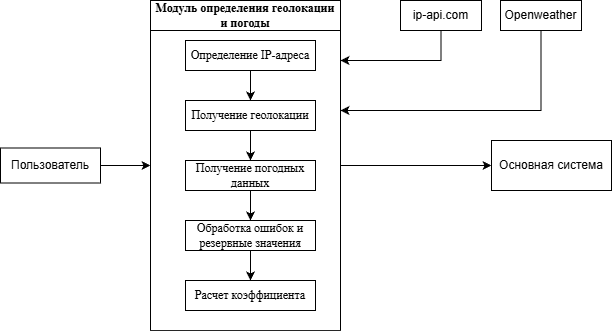
\includegraphics[width=0.9\linewidth]{pics/Picture3}
\caption{Конвейер обработки данных модуля контекстной адаптации}
\end{figure}

Процесс обработки данных включает следующие последовательные этапы:
\begin{enumerate}
    \item \textbf{Идентификация местоположения.} IP-адрес пользователя извлекается из HTTP-запроса и передаётся в RESTful API сервиса \texttt{ip-api.com}~\cite{ipapi2026}. Сервис возвращает JSON-объект, содержащий информацию о стране, регионе, городе, часовом поясе и географических координатах.
    \item \textbf{Получение метеорологических данных.} На основе полученных координат формируется GET-запрос к API \texttt{OpenWeatherMap}~\cite{openweathermap2026}, предоставляющему актуальные данные о температуре, атмосферном давлении, влажности, а также код текущего погодного условия.
    \item \textbf{Обработка ошибок и фолбэк-механизмы.} Модуль реализует трёхуровневую систему отказоустойчивости: (а) повторные запросы при временной недоступности API (retry logic с экспоненциальной задержкой); (б) использование кэшированных значений при превышении таймаута; (в) применение дефолтных региональных коэффициентов при полной недоступности внешних сервисов.
    \item \textbf{Расчёт интегрального показателя.} На основе нормализованных значений $K_{\text{region}}$, $K_{\text{temp}}$ и $K_{\text{weather}}$ вычисляется параметр~$P$ по формуле~\eqref{eq:P}, отражающий текущую предрасположенность обучающегося к эффективной учебной деятельности.
    \item \textbf{Интеграция с основной системой.} Рассчитанное значение~$P$ передаётся через сигнальный механизм Django в модуль адаптивных рекомендаций~\cite{brusilovsky2007usermodels}, где используется как весовой коэффициент при формировании персонализированной учебной траектории, выборе времени проведения аттестационных мероприятий и определении оптимальной сложности учебных материалов.
\end{enumerate} % вторая глава - в файле part2.tex
\pagebreak

% если есть еще разделы - сохраните их в соответствующих файлах и раскомментируйте строки ниже, при необходимости добавьте еще
%\section{Практическая реализация системы}
\label{sec:practical_implementation}

В данном разделе описана практическая реализация интеллектуальной обучающей системы LearnSys, разработанной на основе открытого веб-фреймворка Django~\cite{django2026docs} с использованием языка программирования Python. Система реализована в виде монолитного веб-приложения, архитектура которого подчиняется принципам модульности и разделения ответственности, что обеспечивает высокую сопровождаемость кодовой базы и возможность независимого развития отдельных функциональных блоков.
Система структурно разделена на шесть логических модулей, каждый из которых отвечает за определённый аспект образовательного процесса. Модуль авторинга курсов предоставляет преподавателю инструменты для создания и структурирования учебных материалов, включая визуальный конструктор тем, управление графом зависимостей и настройку психологических параметров контента. Модуль психодиагностики реализует механизмы психологического тестирования обучающихся по методикам EPI и МУН с последующим расчётом четырёх ключевых факторов когнитивного профиля (A1--A4) и формированием агрегированного психологического профиля с персонализированными рекомендациями в формате T/R/C. Модуль адаптивного тестирования обеспечивает динамический подбор заданий на основе однопараметрической модели теории ответов на задания (модель Раша) с итеративным обновлением оценки способности обучающегося методом максимального правдоподобия. Модуль трекинга активности собирает поведенческие данные через отслеживание движений курсора мыши и рассчитывает метрики мотивации и нейротизма, которые интегрируются в психологический профиль студента. Модуль пользовательских интерфейсов включает дашборды для студентов и преподавателей, формы регистрации и авторизации, визуализацию прогресса обучения и графов зависимостей тем. Модуль аналитики предоставляет агрегированные отчёты по успеваемости, поведенческим метрикам и рекомендациям, а также реализует рекомендательный движок, синтезирующий данные когнитивного профиля, поведенческой аналитики и контекстных факторов.
Все модули взаимодействуют через единую объектно-реляционную базу данных, построенную с использованием встроенного ORM-фреймворка Django, и общий слой бизнес-логики, обеспечивающий целостность данных и согласованность работы компонентов. Архитектура системы построена на принципе разделения ответственности (Separation of Concerns), реализованном через архитектурный паттерн Model-View-Template (MVT), являющийся вариацией классического паттерна MVC. Модели данных описывают предметную область системы, включая сущности пользователей, курсов, тем, тестов, психологических профилей и поведенческой аналитики, и обеспечивают декларативное определение структуры базы данных с поддержкой сложных связей (один ко многим, многие ко многим) и ограничений целостности. Представления обрабатывают входящие HTTP-запросы, реализуют бизнес-логику системы, включая адаптивные алгоритмы подбора контента, расчёт психологических факторов и генерацию персонализированных рекомендаций, и возвращают ответы в формате HTML-страниц или JSON-данных для асинхронных запросов. Шаблоны формируют пользовательский интерфейс с использованием языка разметки Django Templates и клиентских библиотек (HTMX для динамического обновления контента без перезагрузки страницы, vis-network для визуализации графов зависимостей, Chart.js для построения интерактивных графиков). Маршрутизация запросов осуществляется через централизованный механизм определения URL-шаблонов, который сопоставляет входящие запросы с соответствующими представлениями и обеспечивает чистые, семантически значимые адреса для всех функциональных эндпоинтов системы.
Дополнительно система включает слой утилитарных модулей, выносящих сложные алгоритмические вычисления за пределы основных представлений. В частности, алгоритмы расчёта психологических факторов, валидации результатов тестирования, генерации рекомендаций и обработки поведенческих данных реализованы в виде независимых функций, что обеспечивает их переиспользуемость и упрощает модульное тестирование. Слой форм обеспечивает валидацию входных данных на стороне сервера, защиту от распространённых уязвимостей (CSRF-атаки, SQL-инъекции, XSS) и унифицированный интерфейс для работы с пользовательским вводом. Система аутентификации и авторизации построена на расширенной модели пользователя, поддерживающей ролевое разграничение доступа (студент, преподаватель, администратор) через специализированные миксины, проверяющие права доступа перед выполнением защищённых операций.
Такая многоуровневая архитектура обеспечивает высокую степень абстракции между компонентами системы, что позволяет независимо модифицировать отдельные модули без влияния на остальные части приложения. Например, замена алгоритма адаптивного тестирования или добавление новой психометрической методики требует изменений только в соответствующем утилитарном модуле и моделях данных, тогда как пользовательский интерфейс и маршрутизация остаются неизменными. Подобная модульность делает систему пригодной для дальнейших научных исследований в области адаптивного обучения, позволяя исследователям экспериментировать с новыми алгоритмами и моделями без необходимости перестройки всей архитектуры.
%=============================================================
\subsection{Реализация модуля авторинга курсов}
\label{subsec:authoring_module}

\subsubsection{Архитектура модели предметной области}

Модуль авторинга курсов является центральным компонентом системы со 
стороны преподавателя. Его архитектура основана на иерархии моделей 
данных, реализованных с помощью ORM Django.

Верхним уровнем иерархии является модель \texttt{Course}, описывающая 
учебный курс. Она содержит следующие ключевые поля:

\begin{itemize}
    \item \texttt{name} --- уникальное название курса (до 255 символов);
    \item \texttt{description} --- краткое описание курса (до 500 символов);
    \item \texttt{content} --- расширенное описание программы и требований;
    \item \texttt{difficulty} --- уровень сложности, принимающий одно из 
          трёх значений: \texttt{'beginner'} (новичок), 
          \texttt{'intermediate'} (средний), \texttt{'advanced'} (продвинутый);
    \item \texttt{is\_published} --- флаг публикации курса, определяющий 
          его видимость студентам;
    \item \texttt{instructor} --- внешний ключ на модель \texttt{User}, 
          указывающий на преподавателя---автора;
    \item \texttt{tags} --- связь многие---ко---многим с моделью \texttt{Tag}, 
          используемая для категоризации курсов и работы рекомендательной 
          подсистемы.
\end{itemize}

Следующий уровень иерархии --- модель \texttt{Topic}, представляющая 
отдельную тему курса. Ключевыми полями являются:

\begin{itemize}
    \item \texttt{course} --- внешний ключ на \texttt{Course} 
          (каскадное удаление);
    \item \texttt{order\_index} --- целочисленный индекс, определяющий 
          базовый порядок тем;
    \item \texttt{is\_visible} --- флаг видимости темы студентам;
    \item \texttt{prerequisites} --- рекурсивная связь многие---ко---многим 
          (\texttt{symmetrical=False}), формирующая ориентированный граф 
          предварительных требований: если тема $B$ имеет в 
          \texttt{prerequisites} тему $A$, то $A$ должна быть изучена 
          прежде $B$;
    \item \texttt{related\_topics} --- симметричная связь многие---ко---многим 
          для смежных тем, рекомендуемых к совместному изучению;
    \item \texttt{psych\_characteristics} --- поле типа \texttt{JSONField}, 
          хранящее психологические параметры темы в виде словаря.
\end{itemize}

\begin{lstlisting}[language=Python, caption={Структура поля psych\_characteristics}, basicstyle=\small\ttfamily]
{
    "pace":        "slow" | "medium" | "fast",
    "structure":   "low"  | "high",
    "interaction": "independent" | "group",
    "stress_level":"low"  | "medium" | "high",
    "challenge":   "low"  | "medium" | "high"
}
\end{lstlisting}

Эти параметры используются адаптационным движком при вычислении 
персонализированного порядка тем для конкретного студента.

Третий уровень --- модель \texttt{TopicContent}, представляющая единицу 
учебного материала внутри темы. Поле \texttt{content\_type} определяет 
тип контента и принимает одно из значений: \texttt{'text'} (текст), 
\texttt{'video'} (видео), \texttt{'quiz'} (тест), \texttt{'file'} 
(файл), \texttt{'image'} (изображение), \texttt{'audio'} (аудио). 
В зависимости от типа заполняются соответствующие поля: 
\texttt{text\_content} (текстовое содержимое), \texttt{video\_url} 
(ссылка на видео), \texttt{content} (загружаемый файл через 
\texttt{FileField}). Поле \texttt{generated\_text} предназначено для 
хранения результата автоматической обработки контента --- транскрипции 
аудио или перевода текста.

\subsubsection{Интерфейс преподавателя}

Интерфейс преподавателя реализован через набор классовых представлений 
(class---based views), наследующих от стандартных обобщённых представлений 
Django. Доступ к функциям авторинга защищён миксином 
\texttt{UserPassesTestMixin}, проверяющим принадлежность пользователя 
к роли преподавателя через функцию \texttt{is\_instructor(user)} из 
\texttt{\_\_init\_\_.py}.

Для создания и редактирования курса используются представления 
\texttt{CourseCreateView} и \texttt{CourseUpdateView}, обрабатывающие 
форму \texttt{CourseForm}. Форма включает поля \texttt{name}, 
\texttt{description}, \texttt{content}, \texttt{difficulty}, 
\texttt{tags} (виджет \texttt{SelectMultiple}) и \texttt{is\_published} 
(виджет \texttt{CheckboxInput}). При успешной валидации представление 
\texttt{CourseCreateView} автоматически устанавливает поле 
\texttt{instructor} в текущего пользователя через метод 
\texttt{form\_valid}.

Создание и редактирование тем реализовано через \texttt{TopicCreateView} 
и \texttt{TopicUpdateView}, использующие форму \texttt{TopicForm}. 
Особенностью этой формы является наличие виртуальных полей для 
психологических параметров, не хранящихся в базе данных напрямую. 
Поля \texttt{psych\_pace}, \texttt{psych\_structure}, 
\texttt{psych\_interaction}, \texttt{psych\_stress\_level} и\\ 
\texttt{psych\_challenge} реализованы как объекты \texttt{ChoiceField} 
с предопределёнными наборами значений. Метод \texttt{clean} формы 
агрегирует выбранные значения в JSON---словарь и сохраняет его в\\ 
\texttt{cleaned\_data['psych\_characteristics']}, который затем 
записывается в поле \texttt{psych\_characteristics} модели \texttt{Topic}.

Фильтрация выпадающих списков \texttt{prerequisites} и 
\texttt{related\_topics} выполняется в методе \texttt{\_\_init\_\_} 
формы: запрос ограничивается темами того же курса (параметр 
\texttt{current\_course}), исключая саму редактируемую тему во 
избежание циклических зависимостей.

\subsubsection{Управление графом тем}

Граф зависимостей тем визуализируется с помощью библиотеки 
vis---network, подключаемой через CDN. Представление 
\texttt{TopicGraphEditorView} формирует JSON---объект, содержащий 
массивы узлов (темы) и рёбер (связи), и передаёт его в шаблон 
через контекстную переменную \texttt{graph\_data\_json}.

\begin{lstlisting}[language=Python, caption={Формирование данных графа тем}, basicstyle=\small\ttfamily]
graph_data = {'topics': [], 'edges': []}
for topic in topics:
    graph_data['topics'].append(
        {'id': topic.id, 'name': topic.name}
    )
    for prereq in topic.prerequisites.all():
        graph_data['edges'].append(
            {'from': prereq.id, 'to': topic.id, 'type': 'prereq'}
        )
    for related in topic.related_topics.all():
        if related.id > topic.id:
            graph_data['edges'].append(
                {'from': topic.id, 'to': related.id, 'type': 'related'}
            )
\end{lstlisting}

Сохранение изменений графа осуществляется через API---представление 
\texttt{TopicGraphSaveAPI}, принимающее POST---запрос с телом в формате 
JSON. Тело запроса содержит два массива: \texttt{prerequisites} (список 
пар \texttt{\{from, to\}}) и \texttt{related\_topics}. Перед применением 
изменений все существующие связи очищаются, после чего восстанавливаются 
из переданного массива.

При включённом режиме 
\texttt{use\_psych\_params} для каждой темы вычисляется показатель 
сложности на основе значений полей\\ \texttt{psych\_characteristics}: 
значение \texttt{'high'} для поля \texttt{challenge} добавляет 3 балла, 
\texttt{'medium'} --- 2, \texttt{'low'} --- 1; аналогично учитывается поле 
\texttt{stress\_level}. Темы сортируются по возрастанию сложности, и 
более простые темы автоматически добавляются в \texttt{prerequisites} 
более сложных. Дополнительно выявляются пары тем с совпадением двух и 
более психологических параметров, которые соединяются как 
\texttt{related\_topics}.

\subsubsection{Автоматизированная обработка контента}

Обработка мультимедийного контента реализована в модуле\\ 
\texttt{utils/content\_processing.py}.Функция
\texttt{process\_content} вызывается после сохранения 
объекта \texttt{TopicContent} в методах \texttt{form\_valid} представлений 
\texttt{TopicContentCreateView} и \texttt{TopicContentUpdateView}.

Для аудиоконтента (\texttt{content\_type == 'audio'}) вызывается 
функция \texttt{transcribe\_audio}, реализованная с возможностью 
подключения модели Whisper~\cite{woolf2009building}. 
Результат транскрипции сохраняется в поле \texttt{generated\_text}. 
Для текстового контента в поле \texttt{generated\_text} копируется 
значение \texttt{text\_content}. В перспективе функция 
\texttt{translate\_ru\_to\_en} обеспечит перевод через MarianMT 
для создания мультиязычных материалов.

Порядок отображения материалов внутри темы определяется полем 
\texttt{order\_index} модели \texttt{TopicContent}. Запрос материалов 
выполняется с сортировкой \texttt{order\_by('order\_index', 'id')}, 
обеспечивающей стабильный детерминированный порядок при равных 
значениях индекса.

%=============================================================
\subsection{Реализация модуля психодиагностики}
\label{subsec:psychodiagnostics_module}

\subsubsection{Структура психометрических тестов}

Модуль психодиагностики реализует методику оценки четырёх 
психологических факторов согласно требованиям ВКР. Для хранения тестов 
используется модель \texttt{PsychTest}, содержащая поля \texttt{name} 
и \texttt{description}. Каждый тест состоит из вопросов, представленных 
моделью \texttt{PsychQuestion} с полями \texttt{text} (текст вопроса) и 
\texttt{factor} (код фактора: \texttt{'A1'}, \texttt{'A2'}, \texttt{'A3'} 
или их производные с суффиксами \texttt{T}, \texttt{R}, \texttt{C}).

Каждый вопрос имеет набор вариантов ответов, описываемых моделью 
\texttt{PsychAnswer}. Поле \texttt{score} хранит числовой балл, 
начисляемый при выборе данного варианта. Результаты прохождения теста 
фиксируются в модели \texttt{PsychTestResult} с полями \texttt{user} 
(внешний ключ на \texttt{User}), \texttt{factor} (код фактора), 
\texttt{result} (числовой результат) и \texttt{date\_taken} 
(автоматическая метка времени).

\subsubsection{Алгоритм расчёта факторов}

Расчёт психологических факторов реализован в функции\\ 
\texttt{calculate\_factors} 
в модуле \texttt{utils/calculate\_factors.py}. Параметр 
\texttt{user\_answers} представляет собой словарь вида 
\texttt{\{question\_id: answer\_id\}}.

Алгоритм выполняется в шесть этапов.

Этап 1: Загрузка вопросов.Загружаются вопросы теста с 
предзагрузкой вариантов ответов через \texttt{prefetch\_related} для 
минимизации числа SQL---запросов.

Этап 2: Накопление баллов. Для каждого вопроса определяется 
выбранный вариант ответа, находится его балл (\texttt{selected\_answer.score}) 
и добавляется к счётчику соответствующего фактора в словаре 
\texttt{factor\_scores}.

Этап 3: Расчёт темперамента.Фактор \texttt{A4} не вычисляется 
непосредственно из ответов, а определяется как комбинация факторов 
\texttt{A2} (экстраверсия) и \texttt{A3} (нейротизм) по кругу Айзенка:

\begin{lstlisting}[language=Python, 
    caption={Определение типа темперамента по кругу Айзенка},
    basicstyle=\small\ttfamily]
if a3_score < 12 and a2_score < 12:
    factor_scores['A4'] = 1   
elif a3_score < 12 and a2_score >= 12:
    factor_scores['A4'] = 2   
elif a3_score >= 12 and a2_score < 12:
    factor_scores['A4'] = 3   
else:
    factor_scores['A4'] = 4  
\end{lstlisting}

\textbf{Этап 4: Ограничение значений.} Значения каждого фактора 
ограничиваются допустимыми диапазонами согласно Таблице~1 ВКР:
\begin{itemize}
    \item \texttt{A1}: диапазон $[0, 20]$ --- шкала мотивации МУН;
    \item \texttt{A2}: диапазон $[0, 24]$ --- шкала экстраверсии EPI;
    \item \texttt{A3}: диапазон $[0, 24]$ --- шкала нейротизма EPI;
    \item \texttt{A4}: диапазон $[1, 4]$ --- тип темперамента.
\end{itemize}

\textbf{Этап 5: Генерация рекомендаций.} Для каждого базового фактора 
вызывается функция \texttt{get\_recommendations\_for\_factor(code, score)} 
из \texttt{psych\_factors.py}. Функция возвращает словарь 
с тремя ключами: \texttt{T} (рекомендация преподавателю), \texttt{R} 
(обратная связь) и \texttt{C} (коммьюнити), а также вспомогательный 
словарь \texttt{levels} с числовыми уровнями (1------3). Значения 
определяются по таблице \texttt{PERSONALIZATION\_RULES}, хранящей 
пороговые диапазоны для каждого фактора.

\textbf{Этап 6: Формирование итогового результата.} Функция возвращает 
расширенный словарь \texttt{final\_results}, включающий как базовые 
значения факторов, так и значения с суффиксами \texttt{T}, \texttt{R}, 
\texttt{C}: например, \texttt{'A1T': 2, 'A1R': 3, 'A1C': 1}.

\subsubsection{Генерация психологического профиля}

Формирование агрегированного профиля реализовано в функции 
\texttt{generate\_psych\_profile(student, test\_results, instructor, request)} 
в модуле \texttt{psych\_utils.py}. Функция принимает объект 
пользователя \texttt{student}, QuerySet результатов тестов 
\texttt{test\_results}, объект преподавателя \texttt{instructor} и 
объект HTTP---запроса \texttt{request} (используется для определения 
геолокации по IP).

Первым шагом выполняется группировка результатов по базовым факторам. 
Для каждого результата из строки \texttt{res.factor} отсекаются 
суффиксы через \texttt{res.factor.rstrip('TRC')}, и из нескольких 
записей с одинаковым базовым кодом выбирается наиболее свежая по 
полю \texttt{date\_taken}.

Вторым шагом применяются погодные коррекции. Из объекта запроса 
извлекается IP-адрес (\texttt{HTTP\_X\_REAL\_IP} или 
\texttt{REMOTE\_ADDR}). По IP определяется город через функцию 
\texttt{get\_geo(ip)} из \texttt{recommender.py}, 
обращающуюся к сервису ip-api.com~\cite{ipapi2026}. Затем вызывается 
\texttt{get\_current\_weather(city)}, запрашивающая API 
OpenWeatherMap~\cite{openweathermap2026}. Оба результата кэшируются 
с помощью Django cache framework: геолокация --- на 3600 секунд, 
погода --- на 1800 секунд. По коду погоды (\texttt{weather\_main}) 
из словаря \texttt{WEATHER\_CORRECTIONS} извлекаются коэффициенты 
коррекции факторов и применяются к значениям с соблюдением 
допустимых диапазонов.

Третьим шагом применяются коррекции активности. Поле 
\texttt{activity\_score} модели \texttt{User} отражает накопленную 
активность студента. При значении $\geq 20$ к фактору \texttt{A1} 
добавляется 2 балла, а \texttt{A3} уменьшается на 1; при значении 
от 10 до 19 \texttt{A1} увеличивается на 1; при значении от 1 до 9 
\texttt{A3} увеличивается на 1.

Результатом функции является объект модели \texttt{PsychProfile}, 
создаваемый или обновляемый через \texttt{get\_or\_create}. Модель 
содержит поля \texttt{factor\_a1}, \texttt{factor\_a2}, 
\texttt{factor\_a3}, \texttt{factor\_a4} (скорректированные значения 
факторов), \texttt{guidance\_A1}------\texttt{guidance\_A4} 
(рекомендации в формате JSON), \texttt{summary\_text} (текстовое 
резюме профиля) и \texttt{chart\_data} (метаданные контекста 
формирования: город, погода, применённые коррекции).

Обновление профиля при сохранении результата теста автоматизировано 
через сигнал Django. Обработчик \texttt{auto\_update\_profile\_factors} 
в \texttt{signals.py} подключён через декоратор 
\texttt{@receiver(post\_save, sender=PsychTestResult)} и при создании 
новой записи \texttt{PsychTestResult} немедленно обновляет 
соответствующее поле \texttt{PsychProfile} студента.

\subsubsection{Интерпретация факторов и рекомендации}

Интерпретация числовых значений факторов выполняется вспомогательными 
функциями.

Интерпретация фактора \texttt{A1} (мотивация) основана на пяти 
диапазонах: $[0, 7]$ --- <<выраженная мотивация на неудачу>>, $[8, 9]$ --- 
<<тенденция на неудачу>>, $[10, 11]$ --- <<мотивация не выражена>>, 
$[12, 13]$ --- <<тенденция на успех>>, $[14, 20]$ --- <<выраженная 
мотивация на успех>>. Интерпретация фактора \texttt{A2} (экстраверсия) 
бинарна: значения $\leq 12$ соответствуют интроверсии, значения 
$\geq 13$ --- экстраверсии. Фактор \texttt{A3} (нейротизм) интерпретируется 
по четырём диапазонам: $[0, 6]$ --- низкий уровень, $[7, 13]$ --- средний, 
$[14, 18]$ --- высокий, $[19, 24]$ --- очень высокий. Фактор \texttt{A4} 
(темперамент) принимает ровно четыре значения: 1 --- флегматик, 
2 --- сангвиник, 3 --- меланхолик, 4 --- холерик.

Для отображения профиля студенту и преподавателю вспомогательная 
функция \texttt{\_build\_grouped\_factors\_from\_profile(profile)} 
формирует словарь с ключами \texttt{'A1'}------\texttt{'A4'}, каждый из 
которых содержит поля \texttt{factor\_name}, \texttt{value}, 
\texttt{max\_score}, \texttt{interpretation}, а также текстовые 
значения рекомендаций \texttt{T}, \texttt{R}, \texttt{C}.

%=============================================================
\subsection{Реализация адаптивного тестирования}
\label{subsec:adaptive_testing}

\subsubsection{Модели данных адаптивного тестирования}

Адаптивное тестирование в системе LearnSys реализовано на основе 
однопараметрической модели теории ответов на задания (Item Response 
Theory, IRT), конкретно --- модели Раша. Каждый вопрос теста 
представлен моделью \texttt{TestItem}, содержащей три параметра IRT:

\begin{itemize}
    \item \texttt{a} --- параметр дискриминативности (по умолчанию 1.0);
    \item \texttt{b} --- параметр трудности (по умолчанию 0.0);
    \item \texttt{c} --- параметр случайного угадывания (по умолчанию 0.0).
\end{itemize}

Вероятность правильного ответа студента с уровнем подготовленности 
$\theta$ вычисляется через метод модели:

\begin{lstlisting}[language=Python, 
    caption={Вычисление вероятности правильного ответа (IRT)},
    basicstyle=\small\ttfamily]
def probability_of_correct_answer(self, theta):
    import math
    logistic = 1.0 / (1.0 + math.exp(---self.a * (theta --- self.b)))
    return self.c + (1 --- self.c) * logistic
\end{lstlisting}

Сессия адаптивного теста фиксируется в модели 
\texttt{AdaptiveTestSession} со следующими полями:
\begin{itemize}
    \item \texttt{user} и \texttt{test} --- идентификаторы студента 
          и теста (уникальная пара);
    \item \texttt{theta} --- текущая оценка уровня подготовленности 
          студента (изначально 0.0);
    \item \texttt{asked\_items} --- связь многие---ко---многим с 
          \texttt{TestItem}, содержащая уже заданные вопросы;
    \item \texttt{current\_complexity} --- текущий уровень сложности 
          сессии: \texttt{'easy'}, \texttt{'medium'} или \texttt{'hard'};
    \item \texttt{finished} --- флаг завершения сессии.
\end{itemize}

\subsubsection{Алгоритм адаптивного подбора заданий}

Представление \texttt{AdaptiveTestView} обрабатывает как GET---запросы 
(отображение следующего вопроса), так и POST---запросы (фиксация ответа). 
Максимальное число вопросов в сессии ограничено константой 
\texttt{MAX\_QUESTIONS = 10}. Возможные уровни сложности заданы 
упорядоченным списком \texttt{COMPLEXITY\_ORDER = ['easy', 'medium', 'hard']}.

\textbf{Выбор следующего задания.} Метод \texttt{select\_next\_item} 
реализует стратегию максимального информационного критерия в упрощённой 
форме: из доступных вопросов (не вошедших в \texttt{asked\_items}) 
выбирается тот, для которого разность $|\theta --- b|$ минимальна, то есть 
задание наиболее близко по трудности к текущей оценке подготовленности:

\begin{lstlisting}[language=Python, 
    caption={Выбор следующего задания по минимуму $|\theta --- b|$},
    basicstyle=\small\ttfamily]
def select_next_item(self, test, session):
    available = test.items.exclude(
        id__in=session.asked_items.values_list('id', flat=True)
    )
    return min(
        available,
        key=lambda x: abs(session.theta --- x.b),
        default=None
    )
\end{lstlisting}

\textbf{Оценка $\theta$.} После каждого ответа уровень подготовленности 
обновляется методом \texttt{estimate\_theta}, реализующим итеративный 
градиентный подъём по логарифмической функции правдоподобия. 
Для каждого заданного вопроса вычисляется отклонение между 
наблюдаемым результатом и ожидаемой вероятностью правильного ответа, 
после чего $\theta$ сдвигается на шаг \texttt{step = 0.1}.

\textbf{Обновление уровня сложности.} После каждого ответа метод 
\texttt{update\_complexity} сдвигает текущий уровень сложности на 
одну позицию: при правильном ответе --- в сторону увеличения 
(\texttt{'easy'} $\to$ \texttt{'medium'} $\to$ \texttt{'hard'}), 
при неправильном --- в сторону уменьшения, с ограничением по 
границам списка.

\subsubsection{Фиксация результата и обновление прогресса}

По завершении сессии (достижение \texttt{MAX\_QUESTIONS} или 
исчерпание доступных вопросов) вызывается метод \texttt{finish\_test}. 
Подсчитывается число правильных ответов, создаётся запись 
\texttt{UserTestResult} с полями \texttt{score}, \texttt{max\_score}, 
\texttt{percentage}, \texttt{is\_passed} и \texttt{completed\_at}. 
Флаг \texttt{is\_passed} устанавливается в \texttt{True}, если 
\texttt{percentage} превышает пороговое значение \texttt{passing\_score} 
теста.

Прогресс темы обновляется через метод \texttt{mark\_test\_completed} 
модели \texttt{TopicProgress}. Метод принимает число правильных ответов 
и общее число вопросов, вычисляет процент выполнения и устанавливает 
статус: \texttt{'completed'} при доле правильных ответов $\geq 50\%$ 
или \texttt{'in\_progress'} в противном случае.

%=============================================================
\subsection{Реализация модуля трекинга активности}
\label{subsec:tracking_module}

\subsubsection{Сбор поведенческих данных}

Трекинг движений мыши реализован на клиентской стороне 
средствами JavaScript. В базовом шаблоне \texttt{base.html} 
для авторизованных студентов автоматически активируется функция 
\texttt{startMouseTracking()}, подписывающаяся на событие 
\texttt{mousemove}.

Координаты курсора записываются в массив \texttt{mousePoints} 
в формате \texttt{[timestamp, clientX, clientY]}. Буфер ограничен 
500 точками. Отправка данных на сервер происходит автоматически 
каждые 30 секунд, а также при закрытии вкладки (событие 
\texttt{beforeunload}). Минимальный порог отправки --- 10 точек.

На стороне сервера API---обработчик \texttt{mouse\_tracking\_api} 
декодирует JSON---тело запроса, извлекает массив точек и конвертирует 
временные метки из Unix---времени в миллисекундах в объекты 
\texttt{datetime}. Обработчик требует аутентификации 
(\texttt{@login\_required}) и принимает только POST---запросы.

\subsubsection{Расчёт поведенческих метрик}

Вычисление метрик реализовано в функции 
\texttt{calc\_motion\_metrics(points)} модуля 
\texttt{mouse\_metrics.py}. Функция принимает список 
кортежей \texttt{(timestamp, x, y)} и возвращает пару значений 
\texttt{(motivation, neuroticism)}.

Алгоритм вычисляет суммарное расстояние \texttt{total\_distance} как 
сумму евклидовых расстояний между последовательными точками и суммарное 
время \texttt{total\_time}. Средняя скорость движения 
$v = \frac{\text{total\_distance}}{\text{total\_time}}$ используется 
для оценки активности студента. Метрика мотивации вычисляется как 
$\min(10, \max(0, 5 + v / 100))$, метрика нейротизма --- как 
$\min(10, \max(0, 5 + v / 200))$. При недостаточном числе точек 
(менее 10) функция возвращает нейтральные значения $(5.0, 5.0)$.

\subsubsection{Интеграция с психологическим профилем}

Результаты трекинга сохраняются в полях \texttt{mouse\_motivation\_score} 
и \texttt{mouse\_neuroticism\_score} модели \texttt{PsychProfile}.\\ 
Флаг \texttt{mouse\_tracking\_completed} устанавливается в \texttt{True} 
после первой успешной обработки данных. Если профиль для студента 
ещё не создан, он создаётся автоматически через \texttt{get\_or\_create}.

Поведенческие метрики отображаются на панели аналитики для преподавателей, 
реализованной в функции \texttt{mouse\_metrics\_dashboard} модуля 
\texttt{views\_analytics.py}. Панель агрегирует данные по всем 
профилям с \texttt{mouse\_tracking\_completed=True} и вычисляет 
средние значения мотивации и нейротизма, а также распределение 
студентов по трём группам: низкий уровень (значение $<3$), средний 
($3 \leq$ значение $< 7$) и высокий ($\geq 7$). Таблица корреляции 
сопоставляет поведенческие метрики с психометрическими значениями 
факторов \texttt{A1}------\texttt{A3} для каждого студента.

%=============================================================
\subsection{Интерфейсы пользователей}
\label{subsec:user_interfaces}

\subsubsection{Дашборд студента}

Дашборд студента реализован в классовом представлении\\ 
\texttt{StudentDashboardView}, наследующем \texttt{TemplateView} 
и защищённом миксином \texttt{LoginRequiredMixin}. Доступ 
к представлению возможен только для пользователей с атрибутом 
\texttt{is\_student=True}, проверяемым через функцию 
\texttt{is\_student(user)}.

Метод \texttt{get\_context\_data} формирует следующие данные контекста.

Для каждого курса, доступного студенту 
через учебные группы, вычисляется прогресс обучения. Процент 
выполнения вычисляется как отношение числа тем со статусом 
\texttt{'completed'} к общему числу тем курса. Средний балл 
определяется по записям \texttt{TopicProgress} данного студента. 
Оценка по пятибалльной шкале вычисляется функцией 
\texttt{five\_point\_grade}: балл $\geq 90\%$ соответствует оценке 5, 
$\geq 75\%$ --- оценке 4, $\geq 60\%$ --- оценке 3, ниже --- оценке 2. 
Результаты агрегируются в список словарей \texttt{course\_stats}.

Психологический профиль передаётся в контекст \\как 
\texttt{psych\_profile} --- объект \texttt{PsychProfile}, отобранный 
через\\ \texttt{order\_by('---created\_at').first()}. При отсутствии 
профиля отображается информационный блок с призывом пройти 
психологические тесты и кнопкой перехода к ним.

На дашборде реализована динамическая 
подгрузка рекомендованных курсов через HTMX (\texttt{hx---get}, 
\texttt{hx---trigger="load"}), вызывающую частичное представление 
\texttt{course\_list\_partial}. Резервным механизмом служит 
JavaScript---функция \texttt{loadRecommendations()}, обращающаяся к 
API---эндпоинту \texttt{api/recommendations/}.

\subsubsection{Дашборд преподавателя}

Дашборд преподавателя реализован в \texttt{InstructorDashboardView}. 
Доступ ограничен пользователями с флагом \texttt{is\_instructor=True} 
через \texttt{UserPassesTestMixin}.

Контекст дашборда включает:
\begin{itemize}
    \item \texttt{courses} --- QuerySet курсов, созданных преподавателем 
          (фильтр \texttt{instructor=user}), с предзагрузкой тегов и тем;
    \item \texttt{groups} --- QuerySet учебных групп, связанных с 
          курсами преподавателя через 
          \texttt{courses\_\_in=courses}, дедуплицированный через 
          \texttt{distinct()};
    \item \texttt{students} --- QuerySet студентов из групп курсов 
          преподавателя;
    \item \texttt{stats} --- агрегированная статистика: число курсов, 
          групп, студентов;
    \item \texttt{recent\_activity} --- список событий за последние 
          7 дней: завершённые тесты (из \texttt{UserTestResult}) 
          и новые участники групп (из \texttt{GroupMember}).
\end{itemize}

Быстрые действия на дашборде реализованы через кнопки перехода к 
созданию курса (\texttt{course\_create}), созданию группы 
(\texttt{group\_create}), списку студентов 
(\texttt{instructor\_student\_list}) и панели метрик мыши 
(\texttt{mouse\_metrics\_dashboard}).

\subsubsection{Управление учебными группами}

Учебные группы представлены моделью \texttt{StudyGroup} с полями 
\texttt{name}, \texttt{description}, \texttt{courses} 
(многие---ко---многим с \texttt{Course}), \texttt{instructor} 
(создатель группы), \texttt{is\_active}, \texttt{max\_students} 
и \texttt{academic\_year}.

Участие студентов в группах управляется через промежуточную модель 
\texttt{GroupMember} с полями \texttt{study\_group}, \texttt{user}, 
\texttt{joined\_at}, \texttt{is\_active} и \texttt{notes}. Уникальное 
ограничение \texttt{unique\_together = ('study\_group', 'user')} 
предотвращает дублирование записей.

Форма \texttt{GroupForm} при инициализации фильтрует список доступных 
курсов через параметр \texttt{current\_instructor}: преподаватель видит 
только собственные курсы. При сохранении формы в методе 
\texttt{form\_valid} представлений \texttt{GroupCreateView} и 
\texttt{GroupUpdateView} предыдущий состав группы удаляется 
(\texttt{GroupMember.objects.filter(study\_group=...).delete()}), 
после чего через \texttt{bulk\_create} создаются новые записи для 
студентов, переданных в POST---параметре \texttt{students}.

\subsection{Управление графом зависимостей тем}
\label{subsec:topic_graph_management}

Одним из ключевых механизмов адаптации образовательной траектории в системе LearnSys является граф зависимостей тем курса. Модель \texttt{Topic} поддерживает два типа связей между темами: направленные предварительные требования (\texttt{prerequisites}) и симметричные связанные темы (\texttt{related\_topics}). Совместное использование этих связей позволяет преподавателю задавать как строгую последовательность изучения, так и рекомендации по совместному освоению материалов.

\begin{figure}[htbp]
\centering
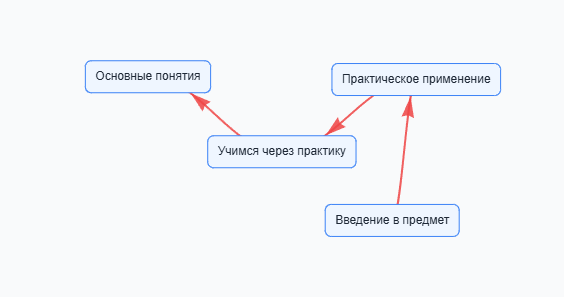
\includegraphics[width=0.85\textwidth]{pics/net.png}
\caption{Граф зависимостей тем, построенный вручную преподавателем}
\label{fig:topic_graph_manual}
\end{figure}

На рисунке~\ref{fig:topic_graph_manual} представлен граф зависимостей тем, созданный преподавателем через визуальный интерфейс конструктора курсов. Красные стрелки отображают направленные связи предварительных требований (\texttt{prerequisites}), заданные вручную через форму \texttt{TopicForm}. Например, связь «Введение в предмет» $\to$ «Практическое применение» означает, что тема «Введение в предмет» должна быть изучена прежде темы «Практическое применение». Аналогично, «Учимся через практику» является предварительным требованием для «Основных понятий» и «Практического применения».

Такой граф формируется преподавателем на основе педагогической логики курса: от простого к сложному, от теории к практике. В модели \texttt{Topic} поле \texttt{prerequisites} реализовано как рекурсивная связь «многие ко многим» с параметром \texttt{symmetrical=False}, что обеспечивает направленность связей. Визуализация графа осуществляется через библиотеку vis---network в представлении \texttt{CourseDetailView}, где данные передаются в шаблон через контекстную переменную \texttt{graph\_data\_json}.

\begin{figure}[htbp]
\centering
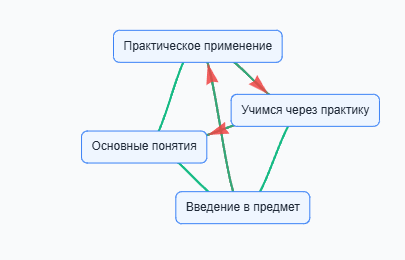
\includegraphics[width=0.85\textwidth]{pics/netauto.png}
\caption{Граф зависимостей тем после автоматического распределения на основе психологического профиля}
\label{fig:topic_graph_auto}
\end{figure}

На рисунке~\ref{fig:topic_graph_auto} показан тот же граф после применения функции автоматического соединения тем \texttt{auto\_connect\_topics}. Помимо исходных красных стрелок (\texttt{prerequisites}), в графе появились зелёные линии без стрелок, представляющие симметричные связи связанных тем (\texttt{related\_topics}). Эти связи формируются автоматически на основе анализа поля \texttt{psych\_characteristics} каждой темы.

Алгоритм работает следующим образом: для каждой пары тем вычисляется показатель схожести по трём психологическим параметрам --- темпу изучения (\texttt{pace}), структуре подачи материала (\texttt{structure}) и типу взаимодействия (\texttt{interaction}). Если две темы совпадают по двум и более параметрам, между ними устанавливается симметричная связь \texttt{related\_topics}. В модели \texttt{Topic} это поле реализовано как связь «многие ко многим» с параметром \texttt{symmetrical=True}, что означает отсутствие направления: если тема A связана с темой B, то и тема B автоматически связана с темой A.

Различие между двумя типами связей имеет принципиальное значение для адаптации траектории обучения. Направленные связи \texttt{prerequisites} (красные стрелки) определяют жёсткий порядок изучения: студент не может перейти к следующей теме, не завершив предварительную. Симметричные связи \texttt{related\_topics} (зелёные линии) носят рекомендательный характер: система предлагает студенту изучить связанные темы совместно или последовательно для более глубокого усвоения материала, но не блокирует переход.

Такой комбинированный подход позволяет системе LearnSys одновременно поддерживать педагогически обоснованную структуру курса, заданную преподавателем, и динамически расширять её рекомендациями на основе психологических характеристик тем. При отображении курса студенту с высоким уровнем мотивации (фактор A1) система может активнее предлагать связанные темы для углублённого изучения, тогда как для студента с высоким нейротизмом (фактор A3) количество рекомендуемых связей сокращается, чтобы снизить когнитивную нагрузку.

\subsection{Структура базы данных системы LearnSys}
\label{subsec:database_structure}

База данных интеллектуальной обучающей системы LearnSys построена с использованием объектно---реляционного отображения (ORM) фреймворка Django и включает пятнадцать основных таблиц, организованных в шесть логических групп. Связи между таблицами реализованы через внешние ключи для отношений «один ко многим» и промежуточные таблицы для отношений «многие ко многим». Полная схема базы данных представлена на рисунке~\ref{fig:er_diagram}.

\begin{figure}[H]  % Вместо [htbp]
\centering
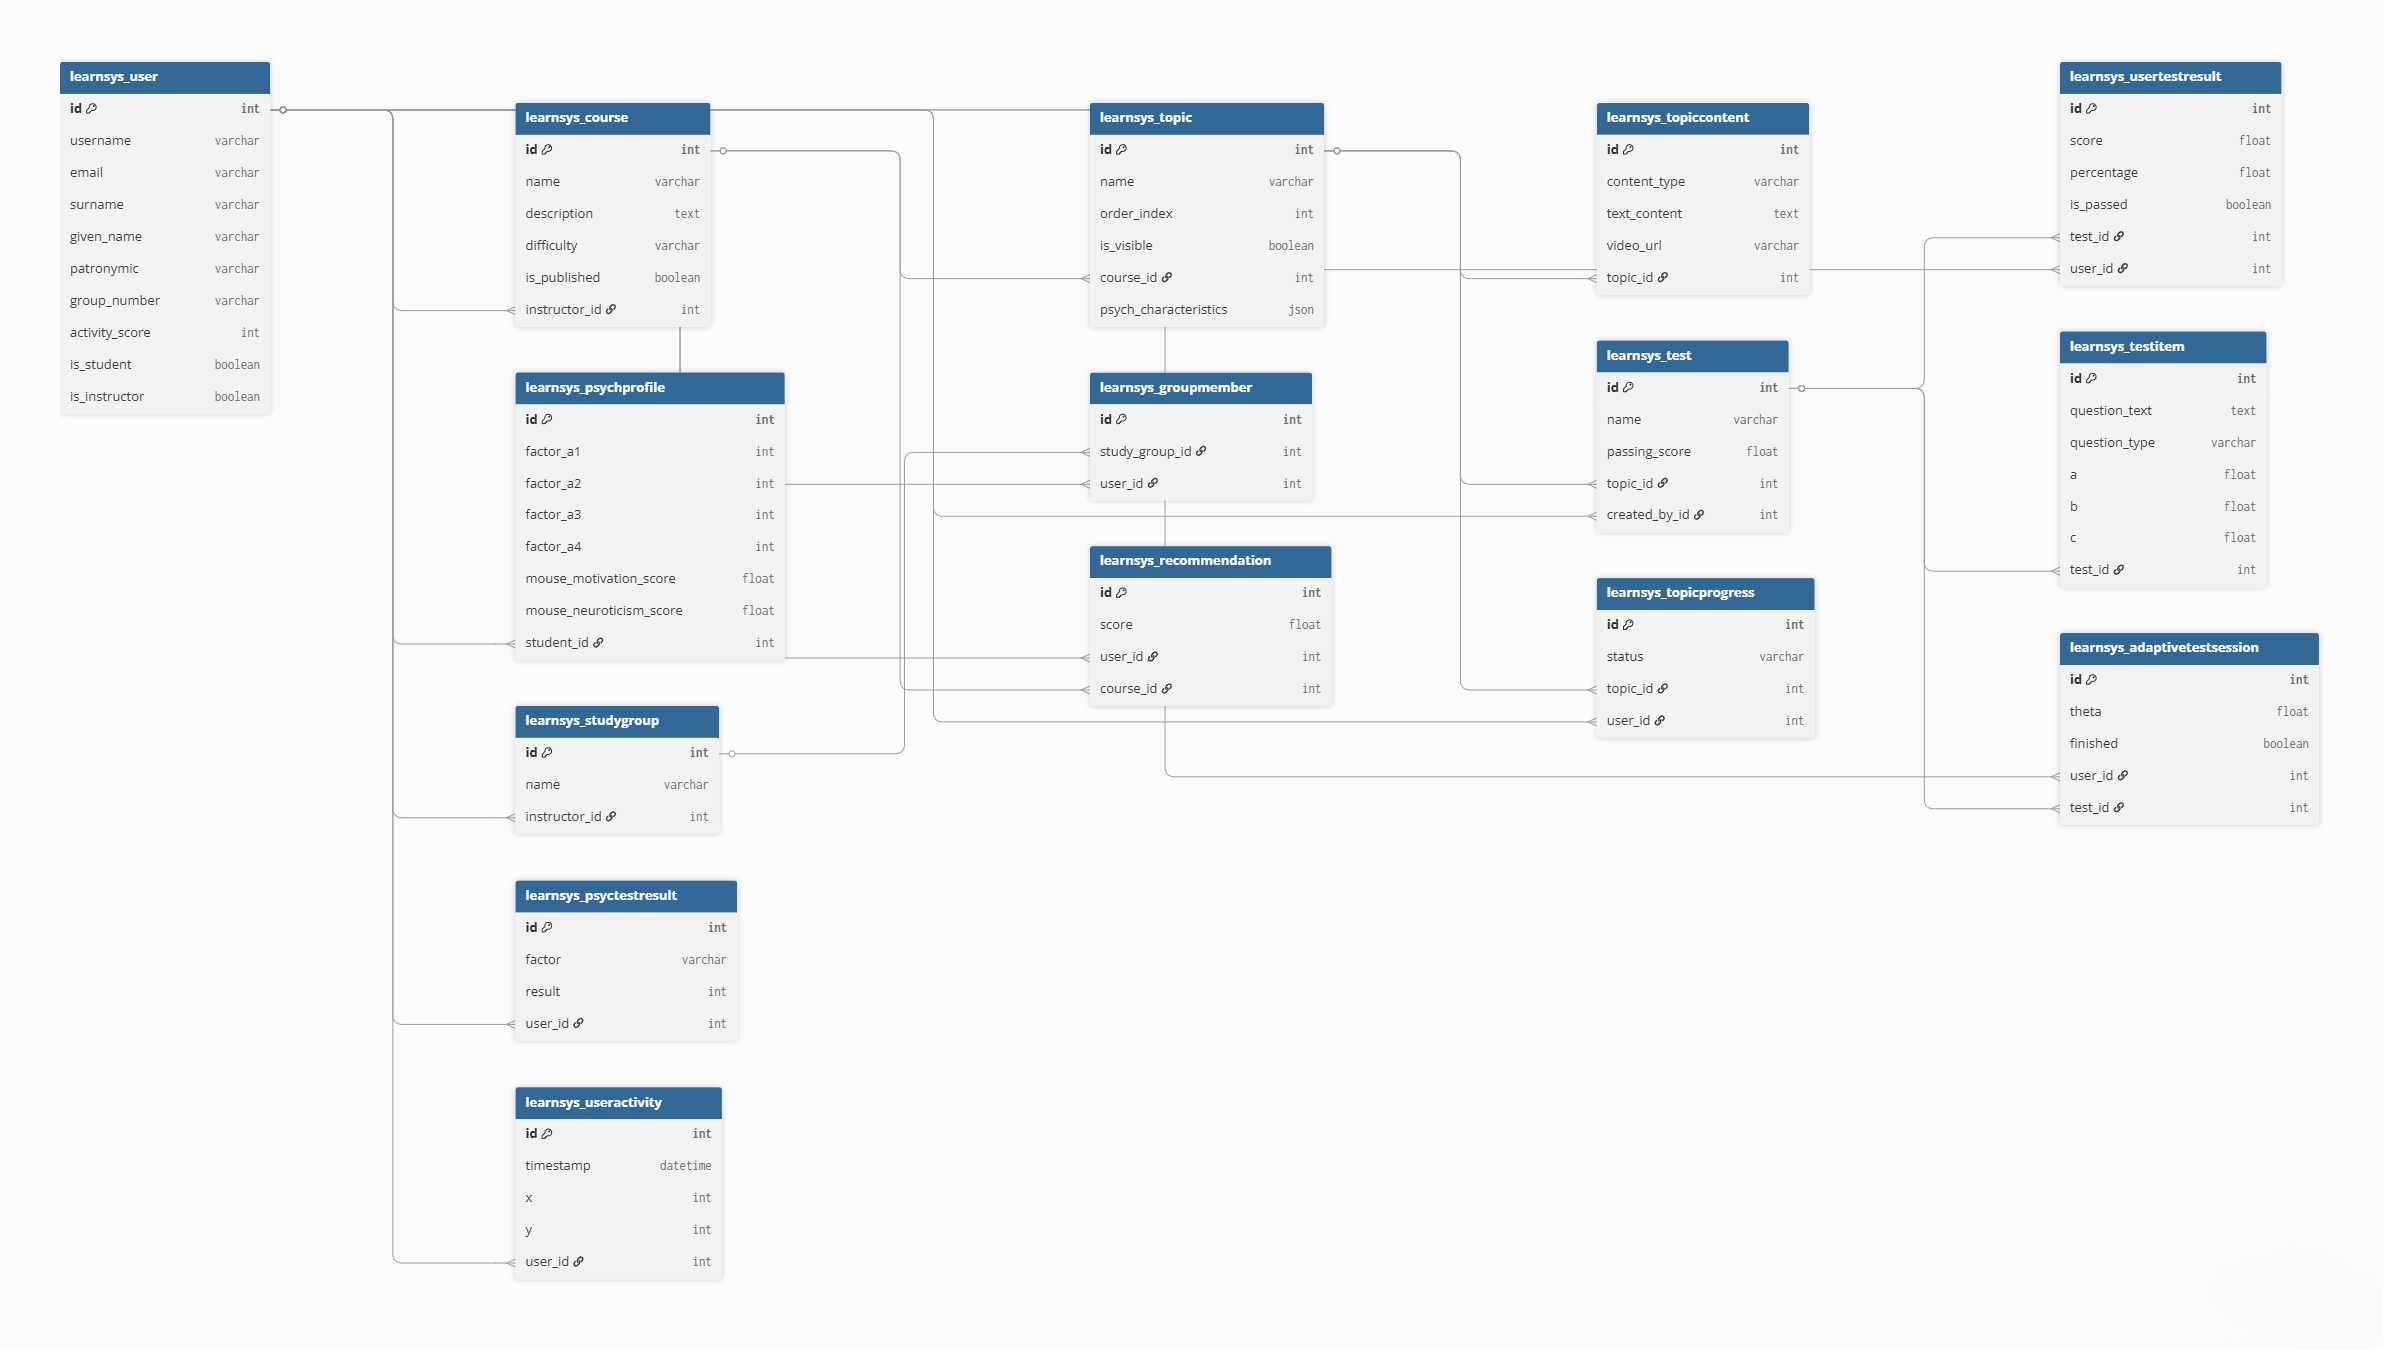
\includegraphics[width=0.95\textwidth]{pics/db.png}
\caption{ER---диаграмма базы данных системы LearnSys}
\label{fig:er_diagram}
\end{figure}

Центральной сущностью системы является таблица \texttt{learnsys\_user}, расширяющая стандартную модель Django дополнительными полями: \texttt{surname}, \texttt{given\_name}, \texttt{patronymic}, \texttt{group\_number}, \texttt{activity\_score}, а также флагами ролей \texttt{is\_student} и \texttt{is\_instructor}. Разграничение прав доступа между студентами и преподавателями обеспечивается на уровне представлений через миксины \texttt{LoginRequiredMixin} и \texttt{UserPassesTestMixin}, которые проверяют принадлежность пользователя к соответствующей роли перед предоставлением доступа к функциональным эндпоинтам.

Группа учебного контента образует иерархию \texttt{Course} $\to$ \texttt{Topic} $\to$ \texttt{TopicContent}. Модель \texttt{Course} содержит поля \texttt{name}, \texttt{description}, \texttt{difficulty} (с тремя уровнями сложности), \texttt{is\_published} и внешний ключ \texttt{instructor\_id} на таблицу пользователей. Модель \texttt{Topic} поддерживает рекурсивные связи \texttt{prerequisites} и \texttt{related\_topics} для формирования графа зависимостей тем, а также поле \texttt{psych\_characteristics} типа JSON для хранения психологических параметров темы (темп, структура, тип взаимодействия, уровень стресса, сложность). Модель \texttt{TopicContent} описывает единицу учебного материала с полем \texttt{content\_type}, принимающим значения текст, видео, аудио, файл, изображение или тест, и полем \texttt{generated\_text} для хранения результата автоматической обработки контента.

Группа тестирования включает модели \texttt{Test}, \texttt{TestItem}, \texttt{UserTestResult} и \texttt{AdaptiveTestSession}. Таблица \texttt{Test} связана с темой курса и содержит параметры прохождения: \texttt{passing\_score}, \texttt{time\_limit}, \texttt{allow\_retake}, \texttt{max\_attempts}. Таблица \texttt{TestItem} хранит вопросы теста с параметрами IRT---модели Раша: дискриминативность \texttt{a}, сложность \texttt{b} и вероятность угадывания \texttt{c}. Таблица \texttt{UserTestResult} фиксирует результаты прохождения теста пользователем: набранные баллы, процент правильных ответов, статус прохождения и время выполнения. Таблица \texttt{AdaptiveTestSession} реализует адаптивное тестирование, храня текущую оценку способности $\theta$ студента, список заданных вопросов и текущий уровень сложности сессии.

Группа психологического профилирования состоит из таблиц\\ \texttt{PsychTestResult} и \texttt{PsychProfile}. Таблица \texttt{PsychTestResult} хранит сырые результаты психологического тестирования с кодом фактора и числовым значением. Таблица \texttt{PsychProfile} является агрегированным профилем студента и содержит четыре ключевых фактора: \texttt{factor\_a1} (мотивация, шкала 0------20), \texttt{factor\_a2} (экстраверсия, шкала 0------24), \texttt{factor\_a3} (нейротизм, шкала 0------24), \texttt{factor\_a4} (темперамент, значения 1------4). Дополнительно в профиле хранятся поведенческие метрики трекинга мыши (\texttt{mouse\_motivation\_score}, \texttt{mouse\_neuroticism\_score}), рекомендации в формате T/R/C для каждого фактора и текстовые выводы для преподавателя и студента.

Группа учебных групп включает модели \texttt{StudyGroup} и \texttt{GroupMember}. Таблица \texttt{StudyGroup} описывает учебную группу с полями \texttt{name}, \texttt{description}, \texttt{academic\_year}, \texttt{max\_students} и внешним ключом на преподавателя---создателя. Таблица \texttt{GroupMember} реализует связь «многие ко многим» между группами и студентами с полями \texttt{joined\_at}, \texttt{is\_active} и \texttt{notes}.

Группа аналитики и рекомендаций представлена таблицами\\ \texttt{UserActivity}, \texttt{TopicProgress} и \texttt{Recommendation}. Таблица \texttt{UserActivity} фиксирует события трекинга активности мыши с временной меткой и координатами курсора. Таблица \texttt{TopicProgress} отслеживает прогресс студента по каждой теме со статусами «не начато», «в процессе», «завершено» и полями результатов тестирования. Таблица \texttt{Recommendation} хранит персонализированные рекомендации курсов для каждого пользователя с числовым показателем релевантности и JSON---полем факторов, использованных при формировании рекомендации.

Все связи между таблицами обеспечивают целостность данных через каскадное удаление и ограничения уникальности. Например, уникальное ограничение \texttt{unique\_together = ('user', 'topic')} в таблице \texttt{TopicProgress} гарантирует наличие не более одной записи прогресса для каждой пары студент------тема, а ограничение \texttt{unique\_together = ('user', 'test')} в таблице \texttt{AdaptiveTestSession} обеспечивает единственную активную сессию адаптивного тестирования для каждого теста.
\subsection{Модуль аналитики и отчётности}
\label{subsec:analytics_module}

\subsubsection{Прогресс студентов}

Прогресс обучения студентов отслеживается через модель\\ 
\texttt{TopicProgress}. Каждая запись хранит связку 
\texttt{user}------\texttt{topic} (уникальная пара), поля статуса 
(\texttt{not\_started}, \texttt{in\_progress}, \texttt{completed}), 
временные метки начала и завершения, а также поля результатов теста: 
\texttt{correct\_answers} и \texttt{total\_questions}. Метод 
\texttt{test\_score\_percentage} вычисляет долю правильных ответов. 
Метод \texttt{mark\_reading\_started} устанавливает поле 
\texttt{started\_reading} при первом обращении к материалам темы.

На странице детальной информации о студенте\\ 
(\texttt{StudentDetailView}) для каждого курса отображаются: 
число завершённых тестов\\ (\texttt{completed\_tests}), средний балл\\ 
(\texttt{average\_score\_percent}), вычисляемый через 
\texttt{Avg('percentage')} Django ORM, и процент прохождения курса. 
Для студента с несколькими курсами вычисляется общий средний 
прогресс (\texttt{overall\_average\_progress}).

\subsubsection{Экспорт результатов}

Экспорт результатов психологического тестирования в формат CSV 
реализован в функции \texttt{export\_psych\_test\_csv}. Доступ к 
функции ограничен суперпользователями и персоналом системы. 
Файл формируется через \texttt{csv.writer} с кодировкой UTF---8 
и включает столбцы: ФИО студента, код фактора, числовой результат 
и дата прохождения. Имя файла генерируется из названия теста с 
заменой пробелов на символы подчёркивания.

Дополнительный экспорт персональных данных студента реализован в 
классе \texttt{DownloadStudentInfoView}, формирующем CSV---файл с 
личными данными и историей результатов тестов выбранного студента.

\subsubsection{Критерии эффективности}

Для оценки результатов эксперимента использовались следующие критерии.

Учебные результаты. Сравнивались средние значения поля 
\texttt{percentage} модели \texttt{UserTestResult} в итоговом 
тестировании. Дополнительно анализировалась динамика прогресса 
через поле \texttt{status} модели \texttt{TopicProgress}: доля тем 
со статусом \texttt{'completed'} в каждой группе.

Вовлечённость.Измерялась через поле \texttt{activity\_score} 
модели \texttt{User} (накопленные баллы активности), число завершённых 
тем, а также данные трекинга мыши: среднее значение 
\texttt{mouse\_motivation\_score} в модели \texttt{PsychProfile}.

Удовлетворённость. Оценивалась по опросникам, заполняемым 
участниками после завершения курса. Вопросы касались удобства 
интерфейса, понятности рекомендаций и субъективной оценки полезности 
адаптации.  % третья глава - в файле part3.tex
%\pagebreak

%\input{part4} % четвертая глава - в файле part4.tex
%\pagebreak

%\input{part5}  % пятая глава - в файле part5.tex
%\pagebreak

\section*{\centering ЗАКЛЮЧЕНИЕ}
\addcontentsline{toc}{section}{ЗАКЛЮЧЕНИЕ}

В ходе проделанной работы была проведена --- описать результаты бурной деятельности по выполнению ВКР, разумно в виде списка выполненных задач.

Разработанная программа позволяет --- перечислить основные функциональные характеристики и особенности, можно в виде списка:
\begin{itemize}
\item выполнено такое-то задание;
\item разработана некоторая система;
\item у работы есть перспективы развития.
\end{itemize}

% оформление библиографии - вариант с БД
\pagebreak

\addcontentsline{toc}{section}{СПИСОК ИСПОЛЬЗОВАННЫХ ИСТОЧНИКОВ}
% ВАЖНО: для корректного отображения в списке литературы ссылок на англ.языке в bibtex-описание источника следует добавить поле 
% langid = {english}
\printbibliography

\pagebreak

\renewcommand{\appendixpagename}{\centering Приложения}

\begin{appendices}
\renewcommand{\thesection}{\Asbuk{section}}
\makeatletter
\renewcommand{\theProgram}{\thesection.\@arabic\c@Program}
\makeatother

% каждое приложение задается следующей командой, нумерация - русскими буквами
\section{\centering } 
% независимая нумерация листингов в каждом приложении
\setcounter{Program}{0}

\begin{MyList}{Часть кода реализации класса HashMapValue}{app1}
\begin{MyCodes}
public class HashMapValue {
	
	protected String filename; 
	protected HashMap<String, String> hashValue = 
	new HashMap<>();
	protected HashMap<String, Boolean> hashKeysFlag =
	 new HashMap<>();
	
	public void setData(String key, String value) {
		hashValue.put(key, value);
	}
	
	public String getData(String key) {
		return hashValue.get(key);
	}
    /* ... */
}
\end{MyCodes}
\end{MyList}

\pagebreak

\begin{MyList}{Пример кода}{app2}
\begin{MyCodes}
код второго приложения
\end{MyCodes}

\end{MyList}
% следующее приложение - раскомментировать команды
%\section{\centering } 
%\setcounter{Program}{0}
%\begin{MyCode}
%код третьего приложения
%\end{MyCode}
%\nopagebreak
%\begin{Program}
%\caption{Еще пример кода}\label{app3}
%\end{Program}

\end{appendices}

\end{document}          

